\section{Gadolinium: as a Neutron Converter Material}
%\label{chap:GdFoil}

%%----------------------------------------------------------------------
%%----------------------------------------------------------------------
%\section{Gadolinium}

%Introduction to Gd
Gadolinium (Gd) is a chemical element with atomic number 64. It is a metal and appears as a solid under standard pressure and room temperature. In nature Gd occurs as a composition of seven isotopes; the most abundant being Gd-158 (24.84\%), followed by Gd-160 (21.86\%), Gd-156 (20.47\%), Gd-157 (15.67\%) and Gd-157 (14.80\%).

%Gd Cross section and its use
Gd has many favorable characteristics allowing an eclectic range of use; for instance in alloys to make magnets, electronics and data storage disks( *); and as a contrast agent in MRI, to diagnose cancerous tumors(*).
Of particular interest is its high neutron absorption cross section, high probability of neutron capture. Of all known natural occurring nuclei, Gd-157 has the highest neutron absorption cross section having resonance at thermal-neutron energies (*). As efficient neutron absorbers, Gd plays an important role in neutron shielding alloys for nuclear reactor safety and storage (*). An additional use of great Gd neutron capture is as Gd-based neutron poison, for instance Gd(III) nitrate in moderator systems for regulating power generation and shut-down of Heavy Water Nuclear Reactors (* page 31).
Not limited to the field of nuclear physics, Gd neutron absorption capability also benefit(s?) neutron capture therapy for cancer treatment and neutron detection, due to reaction products following neutron capture.  In gadolinium neutron capture therapy (GdNCT) a cancer patient is injected with Gd endused tracer followed by exposure to a neutron beam. Neutron absorbed by the Gd tracer produce secondary particles such as photons and electrons. While traversing tissue, the particles deposits dose and The particles travels the tissue exposed to a neutron beam, once Gd absorbs neutrons, decays and release product particles the particles  is injected to the cancer patient product particles deposits dose locally to

%Introduction to neutron detection???

%Neutron capture in gadolinium
Neutron capture cross section of natural Gd is given by the weighted sum of isotopic cross sections. Relative abundance of Gd isotopes in natural Gd and their neutron capture cross section are listed in table 1. Isotopes Gd-157 and Gd-155 collectively contribute 99.99\% of the cross section, resulting in 48800±150 barns. Natural Gd interaction with thermal neutrons may therefore be simplified as a “two-absorbing isotope system” consisting of the isotopes Gd155 and Gd157 [Dumazert, 2018].

%Nuclear reaction equation ...

Since natural Gd interaction with neutrons can be ascribed to isotopes Gd-157 and Gd-155, it is worth studying their corresponding nuclear reaction equation.

\begin{equation}
    _{64}^{155}Gd \rightarrow _{64}^{156}Gd^* \rightarrow _{64}^{156}Gd + \gamma + ICe^-     (Q=8.5 MeV)
\end{equation}
\begin{equation}
    _{64}^{157}Gd \rightarrow _{64}^{158}Gd^* \rightarrow _{64}^{158}Gd + \gamma + ICe^-    (Q=7.9 MeV)
\end{equation}

Once a Gd nuclei has absorbed a neutron it exists in an excited energy state from which it decays by gamma-transition, resulting primarily in gamma-ray ($\gamma$-ray) emission and internal conversion (IC) electrons. Byproducts of the decay are Auger and Coster-Kronig (ACK) electrons and X-rays, prompted by vacancies left by the IC electrons, for further explanation of gamma-transition see section ??. The Q-value ($Q$) is defines as the difference in mass before and after a nuclear reaction and represents the net energy released when the nuclei has decayed completely. This energy is distributed as kinetic energy among product particles. Due to the Gd nuclei’s large mass, compared to a photon (massless) and an electron, the recoil energy is neglectable ( Modern Nuclear Chemistry, page 219*). I.e. most of the Q-value is distributed among gamma-rays and IC electrons.


\subsection{Reaction Energy Spectrum}
The excitation energy is distributed among reaction products; 99\% of the energy is carried by prompt gamma-rays and 1.8\% by IC electrons [?,?]. The energy spectrum ranges from 0 to the Q-value of the nucluear reaction. Energies of prompt gamma-rays lie all over the spectrum, while energies of IC electrons and their biproducts are mainly located at the lower end, below 0.2 MeV.

The resulting spectrum is an overlap of two basic components. The first is a continuous spectrum generated by prompt gamma-rays, in the medium to high energy range. The second is a set of discrete lines produced by low energy prompt gamma-rays, IC electrons, Auger electrons and X-rays. In other words, prompt gamma-ray emission add to both the discrete and continuous component, while the remaining reaction products supply the discrete component.
\begin{figure}[h]
\centering
	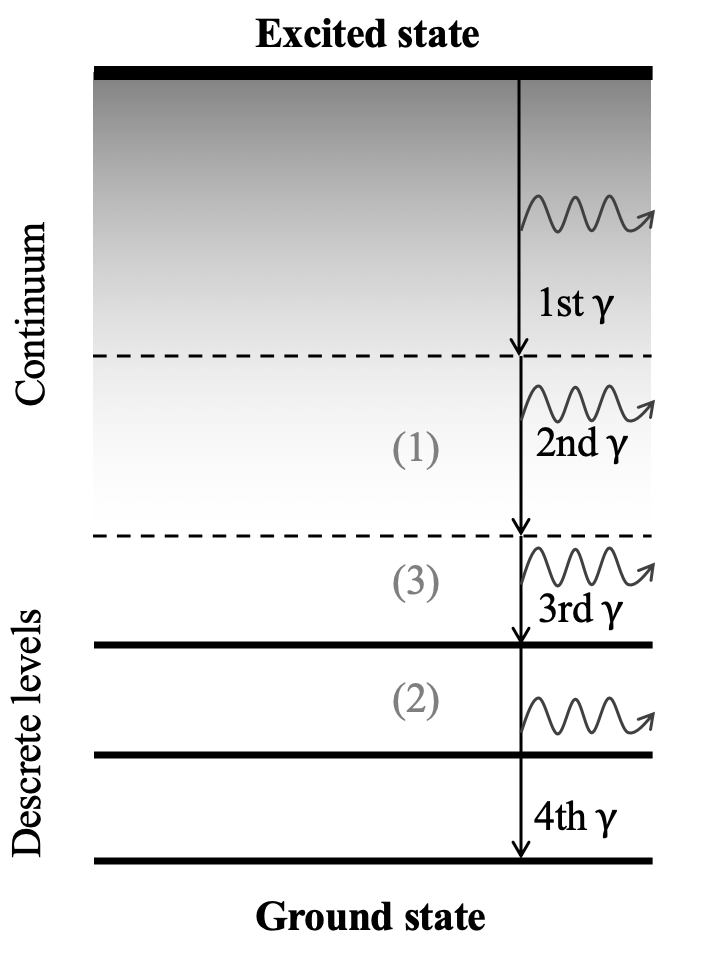
\includegraphics[width=7cm]{/Users/lena/Desktop/Thesis/fig/lvl.png}
	\caption{Nuclear levels of an arbitrary nucleus}
	\label{fig:1}
\end{figure}
The spectrums form is closely related to the arrangement of Gds nuclear levels.
Figure ? illustrates excited states of an arbitrary nucleus. A low lying level have less excitation energy than a high lying level. Low lying levels are easily distinguishable, each with a known spin and parity, they are discrete. As the excitation energy increases so does the nuclear level density, until high lying levels eventually become indistinguishable from one another and resemble a continuum. In fig. ?, the quasicontinuum domain of energy states is represented by a gradient, where energy level density increases as the gradient darkens. Energy levels within the quasicontinuum are marked by dotted lines and the discrete domain with uninterrupted lines. There is no clear boundary between the continuous and discrete domain, but rather a smooth transition between the two. The highest energy level represents neutron capture state and the lowest level ground state, both are indicated by a bold uninterrupted line. A transition from one level to another is indicated by and arrow.

\subsubsection{Prompt Gamma-rays}
%REWRITE!!!
A nucleus may transition once or several times before it reaches ground state.
Transitions can occur between (1) states in the continuous domain, (2) states in the discrete domain or (3) between the two. It is the transitions from initial states in the quasicontinuum that bring about the spectrum’s apparent continuity. Since there are endless state from which a nucleus can decay The domain has an endless number of states , thus giving the gamma endless possibilities of emission energies.

%MISSING Discrete

\subsubsection{Internal Conversion Electrons}
%\textbf{Internal Conversion Electrons}\\
A competing process to gamma-ray emission is internal conversion (IC), the direct emission of an orbital electron. The relationship between the two decay-modes is expressed by the internal conversion coefficient (ICC) $\alpha$. The coefficient is defined as the ratio of IC decay rate $\lambda_{ICe^-}$ to gamma decay rate $\lambda_{\gamma}$:

\begin{equation}
    \alpha =  \frac{\lambda_{ICe^-}}{\lambda_{\gamma}}
\end{equation}

In cases where gamma decay is preferred the coefficient is small, perhaps even negligible, and differently when IC is preferred the coefficient is large. The probability of IC depends on the electron shell (K,L, M, …), there for each shell has its own ICC ($\alpha_K$,$\alpha_L$,$\alpha_M$, …) .
The total ICC is the ratio of total number of IC electrons to gamma-rays emitted by a nucleus and it can be expressed as a sum of shell coefficients:

\begin{equation}
    \alpha_{TOT} =  \sum_i \alpha_i \ , \ i = K, L, M, ...
\end{equation}

%%----------------------------------------------------------------------
%%----------------------------------------------------------------------
